% !TEX root = ../../main.tex
\section{Change Detection}\label{sec:method_change_detection}
In the following sections we haved discussed what data is used for the model construction how the model is interpreted in the context of change detection.
In this section we discuss the methods applicable to the extracted radius $R$ of the hypersphere, in order to indicate a change in the underlying distribution properties.
This employs the second stage of our algorithm, analogue to the second stage of the unifying framework by Takeuchi and Yamanishi~\cite{takeuchi2006unifying}.

In the previous sections we have discussed how a multi-dimensional signal can be reduced to a single dimension time series data based on the radius $R$.
We have argued that in the case of a change in the underlying data, where it becomes more heterogeneous, we expect an increase in the radius $R$.
In the same manner we expect that when the change is in the oldest data objects of the working set the radius $R$ will decrease, since the data becomes more homogeneous.
An abstract representation of these expectations is illustrated in Figure~\ref{fig:radius_expectation}.

\begin{figure}
  \centering
    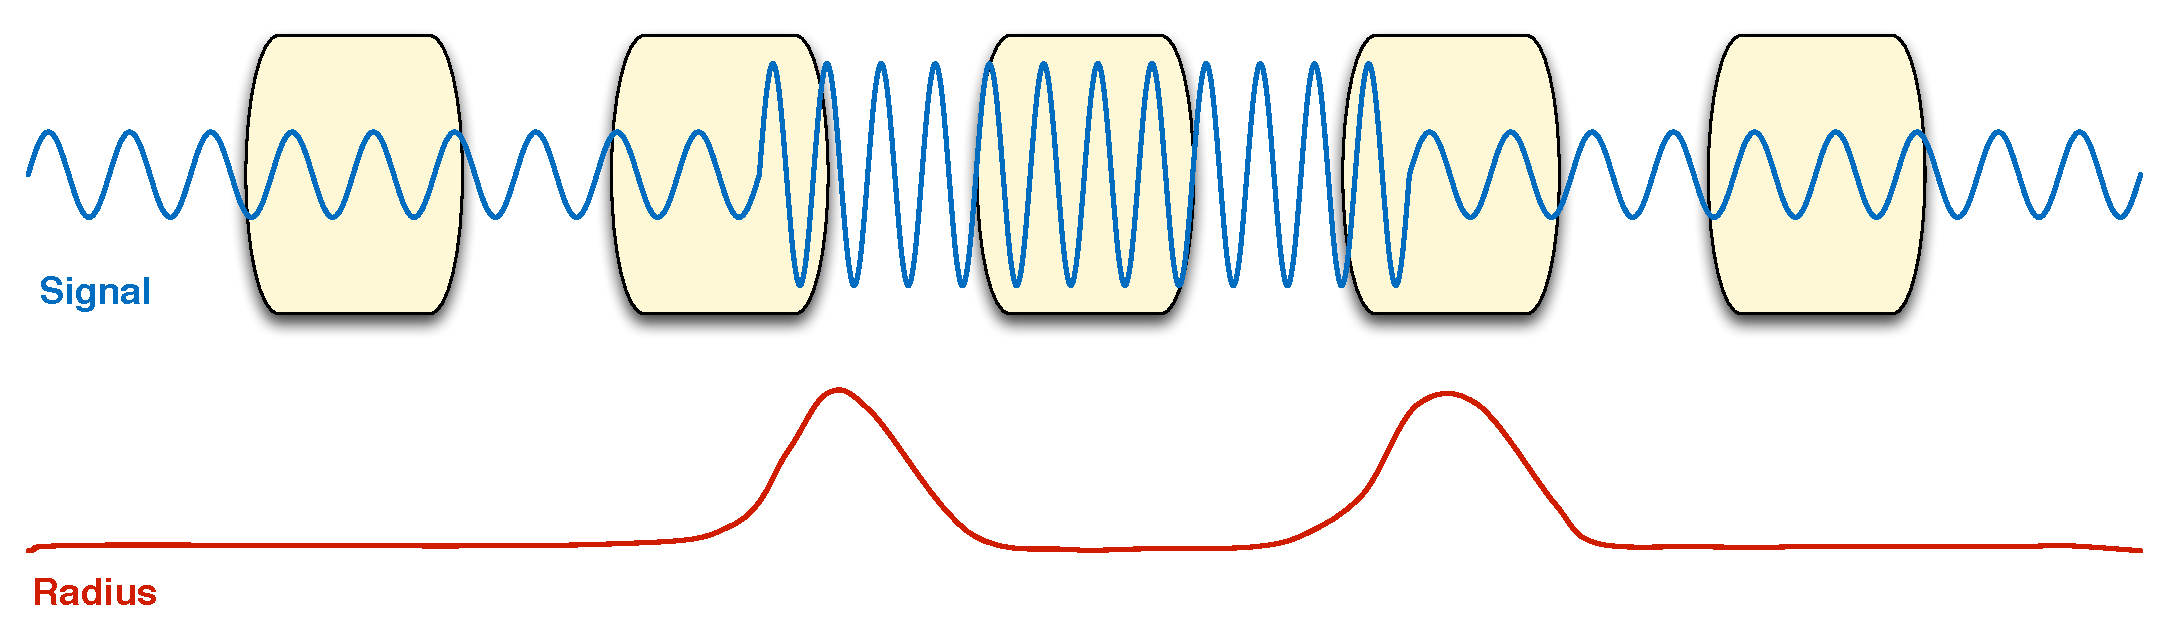
\includegraphics[width=\textwidth,height=\textheight,keepaspectratio]{./Figures/chapter4/expected_behaviour.pdf}
  \caption[Expected radius behaviour]{Expected behaviour of the radius $R$ of the hypersphere. The upper part shows a typical sinusoidal time series signal. The lower graph visualizes an abstract expectation of the values of $R$. Five possible windows are illustrated. The left, middle, and right windows cover an area of homogeneous signal. The expected value of $R$ is low. The other two windows cover a change entering and leaving the window, respectively. At these locations the radius $R$ is expected to increase temporarily. }
  \label{fig:radius_expectation}
\end{figure}

The problem of change detection in complex multi-dimensional time series is now reduced to finding change in a one-dimensional time series.
Besides the dimensionality reduction, the form of the signal is also simplified.
Whereas the original signal was represented as a sinusoidal or second order \gls{ar} model, the new time series is of much simpler form.
In our method we leave open the precise method which is used to find change points in the obtained change indication values.
Below, we will gives two examples of methods which can be applied.
The first example is a ratio-based thresholding mechanism used by Camci~\cite{camci2010change}.

\subsection{Ratio-thresholding}

\begin{equation}\label{eq:ratio_radius}
  \hbar_t = \frac{r_t}{\operatorname*{mean}(r_{y:t-1})},
\end{equation}
where $r_t$ is the approximated radius of the hypersphere at time $t$, $y$ is the time of the last change point (or $1$ if there is non) and $\operatorname*{mean}(r_{y:t-1})$ is the average of the previous approximated radii.